\chapter{AcCAPPCHA}\label{chapter:AcCAPPCHA}
Analysing the structure of Invisible CAPPCHA in \myref{Chapter}{chapter:InvisibleCAPPCHA} and the sensor-based keyloggers in \myref{Section}{sideCH:remote}, I design a CAPTCHA that works approximately like a keylogger. A keylogger is usually a malicious program, used to acquire information about the user's activity by exploiting side-channel information. Its implementation depends on the party, that the hacker wants to attack\cite{keylogging}:
\begin{itemize}
\descItem{The user}
{these attacks are based on the exploitation of physical information related to the typing state. For example, they can use electroencephalography (EEG), motion of the wrist in the smartwatches, video with keyboard line-of-sight and WiFi signal distortion.}
\descItem{The keyboard}
{these attacks are based on the analysis of the signals generated by the keyboard. For example, acoustic emanations can be exploited by using external physical sensors.}
\descItem{The host}
{these attacks are based on the physical access of the attacker to the victim machine. For example, the process footprint, the CPU load and other micro-architectural analysis can be exploited in these attacks.}
\descItem{The network}
{these attacks exploit the packets exchanged in the communication between the client and the server. For example, a network packet can be related to a keystroke revealing the key press time of the victim and the payload size of the server response.}
\end{itemize}
I design a new CAPTCHA based on a keylogger that analyses the keyboard. Considering also the Bio-CAPTCHA voice-based Authentication described in \myref{Section}{soa:Bio_CAPTCHA}, I decide to leverage the audio signal of the microphone of the device. The developed CAPTCHA is called AcCAPPCHA that stands for "Acoustic CAPPCHA". It works in background during the authentication phase, like Invisible CAPPCHA, and it leverages the acoustic side-channel available through the device microphone.
This sensor was chosen to simplify the usability of a CAPPCHA, because it requires only the access permissions to it, without affecting the strength of its bot detection.\\
The whole implementation was made using \texttt{Python} language. The structure and the behaviour of AcCAPPCHA are similar to the ones proposed in Invisible CAPPCHA because they are both based on the analysis of some signal, detected by some sensor, during the insertion of the password.\\
The main difference is that the signal analysed by AcCAPPCHA is generated by the microphone, instead of the accelerometer. However AcCAPPCHA introduces also the analysis of the audio signals using neural networks.\\
According to the sequence of actions performed by Invisible CAPPCHA, AcCAPPCHA performs two steps for the authentication of a user:
\begin{itemize}
\item{Evaluation of the user's activity}
\item{Communication with the remote service}
\end{itemize}
A detailed description of them is reported in the following sections.

\section{Evaluation of the user's activity}\label{AcCAPPCHA:user_activity}
During the evaluation of the user's activity, AcCAPPCHA records two audio signals: the first one created during the insertion of the password and the second one created before. The first signal will be analysed to find the audio peaks. The second signal is exploited to define a threshold, that will be used to find significant audio sequences in the first signal. It was introduced to manage background noise during the classification of the audio. AcCAPPCHA performs two types of verification of the user identity:
\begin{itemize}
\descItem{Time correspondence}{it always requires that the time instants, in which all the characters of the password were typed by the user, are stored. Then an algorithm checks if there exists a sequence of time peaks, observed in the first audio signal, that overlaps with stored time instants. If the sequence exists, the insertion was performed by a human, otherwise by a bot.}
\descItem{Character correspondence}{it doesn't require to store the time instants like in the previous case because it analyses only the first audio signal by labelling each audio peak with a key of the keyboard. Hence AcCAPPCHA checks if there exists a sequence of labels, sorted by increasing time instants, that is equal to the sequence of characters of the password. If the sequence exists, the insertion was performed by a human, otherwise by a bot. The character correspondence could be also done after the application of the time correspondence. In this case, the only differences are:
\begin{itemize}
\item{AcCAPPCHA needs to store the time instants, in which all the characters of the password were typed by the user, to perform time correspondence}
\item{Time correspondence must return the audio peaks that overlap with the stored time instants}
\item{If the time correspondence had positive response, the character correspondence will be applied only on overlapping audio peaks. Otherwise, AcCAPPCHA tells that the insertion was performed by a bot.}
\end{itemize}
The combination of the two verification approaches is more accurate and stronger against false positives (bot detected as human) than the application of only character correspondence.}
\end{itemize}
In the following sections the previous techniques will be explained in details to understand better their pros and cons.   

\subsection{Time correspondence}\label{AcCAPPCHA:time_correspondence}
The first step of the algorithm is the definition of the noise threshold and it's performed before the application asks the user to type the password and after the insertion of the username. During this phase AcCAPPCHA records an audio file of 2 seconds, called \texttt{noise signal}, from the built-in microphone of the laptop and analyses it. The program looks for the maximum value of the audio signal, called $\mathtt{T_N}$, that will be used later during the thresholding phase.\\
The next steps of the verification are performed by two threads simultaneously, during the password insertion. The first thread manages the insertion of the password and it's continuously waiting for the insertion of a character by the user until carriage return ($\mathtt{\setminus r}$) is typed. Immediately after a key is pressed, the time instant of this action, related to the Epoch of the PC, is stored by AcCAPPCHA. The sequence of time instants stored by the thread is called $x=(x_0, ..., x_{|password|-1})$.\\
Meanwhile the second thread records an audio signal, called \texttt{user activity}, using the built-in microphone. The recording session begins immediately after the insertion of the username and it ends after the detection of the carriage return by the first thread. The timestamp of the carriage return isn't stored by AcCAPPCHA and $\mathtt{\setminus r}$ is not considered as part of the password string.\\
Once the above described pieces of information have been acquired, the application has everything it needs to understand if the user is a human or not. In fact the verification is performed by looking if there exists a sequence of audio peaks in the signal that overlaps with the series of the time instants stored by the first thread.\\
First of all, AcCAPPCHA performs the thresholding phase: \texttt{user activity} is analysed by keeping only the samples with values higher than $\mathtt{T_N}$. All the previous operations are performed also in the verification of the character correspondence (see \myref{Section}{AcCAPPCHA:char_correspondence}). The samples, survived after the thresholding, will be grouped in several disjoint windows of maximum width equal to $window\_size$ ms. For each group $W_i$, the application looks for the sample with the highest value, $peak_i$. For example, given the \textit{sampling period} or  \textit{interval} $t_s$ and a specific group of samples: $$W_i = (w_t, w_{t+t_s}, ..., w_{t+\lceil \frac{window\_size}{t_s}\rceil * t_s})$$
the application computes the time instant of the sample related to $peak_i$, $t_i= argmax(W_i)$.\\
Given the sequence of computed time instants $t=(t_0, t_1, ..., t_{n-1})$, related to peaks of all the windows, $n$ the number of windows obtained after thresholding and $|password|$ the size of the password, there is a \textbf{time correspondence} if there exists a subset of $t$, called $t^{*}=({t^*}_0, {t^*}_1..., {t^*}_{|password|-1})$, that matches with the sequence of time instants stored during the password insertion. \myref{Algorithm}{AcCAPPCHA:time_algorithm} is used to find a time correspondence and to establish if the password was inserted by a human or not. The procedure evaluates the distances between the time instant of the first audio peak and the time instants of the other ones. AcCAPPCHA finds a time correspondence if there exists an overlap of the time instants of the audio peaks and the stored time instants with respect to a tolerance factor $threshold$. After several tests, the $window\_size$ of each group $W_i$ and $threshold$ were set respectively to 50 ms and 100 ms (see Section \ref{Results:human}).\\ 
\begin{algorithm}[h]
\DontPrintSemicolon\footnotesize
\KwIn {$\mathtt{x =(x_0, x_1,..., x_{|password|-1})=}$ time instants stored by first thread\newline
$\mathtt{t =(t_0,t_1,...,t_{n-1})=}$ time instants relative to peaks of each group\newline
$\mathtt{threshold=}$ threshold with respect to stored time instant\newline}
\KwOut {$\mathtt{true}$ if human, $\mathtt{false}$ otherwise\newline}
\BlankLine
$\mathtt{y =(y_0, y_1,..., y_{|password|-1})}$ where $y_i=x_i-x_0$\;
\BlankLine
\If{$n<|password|$}{
\textcolor{commentAlg}{//Number of found peaks lower than number of characters of the password}\;
    \BlankLine
    \Return $false$\;
    \BlankLine
}
\BlankLine
\textcolor{commentAlg}{//Search of sequence}\;
\For{$i\leftarrow 0$ \KwTo $n-1$}{
\BlankLine
 \If{$(n-i)<|password|$}{
 \textcolor{commentAlg}{//Not enough peaks after $t_i$ to be analysed to find the time correspondence}\;
    \BlankLine
    \Return $false$\;
    \BlankLine
 }
 \BlankLine
 \textcolor{commentAlg}{//$t_i$ already verified}\;
 $\mathtt{j\gets} i+1$\;
 $\mathtt{count\gets} 1$\;
 \BlankLine
 \While{$count < |password| \wedge j < n$}{
  \BlankLine
  \If{$(n-j)<(|password|-count)$}{
   	\textcolor{commentAlg}{//Not enough peaks after $t_i$ to be analysed to find the time correspondence}\;
   \BlankLine
   $\mathtt{break}$\;
   \BlankLine
  }
  \uIf{$\mathtt{(t_j-t_i)}<(y_{count}-threshold)$}{
   	\textcolor{commentAlg}{//Too less time between the time instant $t_i$ and $t_j$ to obtain time correspondence ($t_j=t_{j+1}$)}\;
    \BlankLine    
    $\mathtt{j}\gets j+1$\;
    \BlankLine
  }
  \uElseIf{$\mathtt{(t_j-t_i)}<(y_{count}+threshold)$}{
	\textcolor{commentAlg}{//Time correspondence}\;
    \BlankLine
    $\mathtt{count}\gets count+1$\;
    $\mathtt{j}\gets j+1$\;
    \BlankLine
  }
  \Else{
   	\textcolor{commentAlg}{//Too much time between the time instant $t_i$ and $t_j$ to obtain time correspondence ($t_i=t_{i+1}$)}\;
    \BlankLine
    $\mathtt{break}$\;
    \BlankLine
  }
  \BlankLine
  \If{$\mathtt{count =} |password|$}{
    \textcolor{commentAlg}{//Time correspondence found}\;
   \BlankLine
   \Return $true$\;
   \BlankLine
  }
  \BlankLine
 }
}
 \caption{Time correspondence}\label{AcCAPPCHA:time_algorithm}
\end{algorithm}
\clearpage
\begin{figure}[h]
     \centering
	 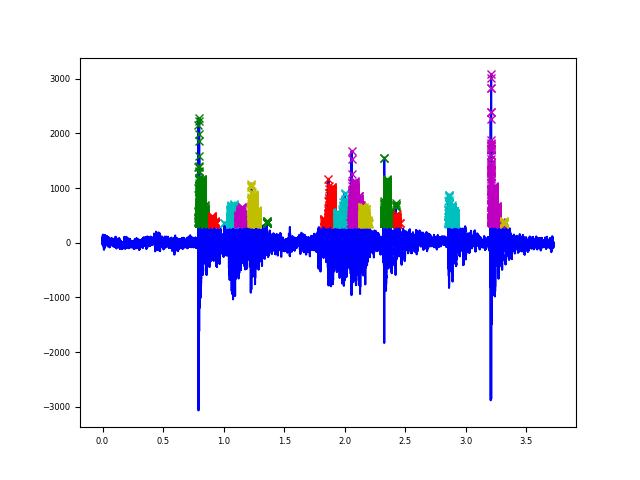
\includegraphics[width=0.8\textwidth]{Images/AcCAPPCHA/hello35_time}
     \caption{\footnotesize{Audio during insertion of password \texttt{hello35} all sub-windows highlighted.}}\label{AcCAPPCHA:hello35_time}
\end{figure}
According to the tests performed, I decided also to relax the problem that time correspondence needs to solve. Given a percentage value $X$, inserted as a command line argument, the algorithm was reformulated in the following way: a user is classified as a human if the time instants of at least $X$\% of the detected audio peaks overlay stored timestamps from keyboard events. According to the results in Section \ref{Results:human}, the percentage $X$, that guarantees the best results in the detection of humans activities, was 90\%.

\subsection{Character correspondence}\label{AcCAPPCHA:char_correspondence}
The character correspondence also looks for audio peaks during the insertion of the password. The identification of the peaks is performed by using two threads as mentioned in time correspondence (see \myref{Section}{AcCAPPCHA:time_correspondence}). The thresholding parameters are obtained in the same way, by exploiting the noise peak, but character correspondence also analyses the shape of the audio signal recorded during the insertion of the password.\\
When a key is pressed by a user on the keyboard, it produces a variation of the audio signal, called \textit{press peak}, for a time window of about 8-10 ms\cite{keyboard_acoustic}. This signal shape in each window can also be divided in three consecutive areas:
\begin{itemize}
\descItem{touch peak}{peak in a window of 2-3 ms, caused by the user's finger touching the key}
\item{\textbf{background noise}}
\descItem{hit peak}{peak in a window of 2-3 ms at the end of the 8-10 ms window, caused by the finger and the key hitting the keyboard supporting plate.}
\end{itemize}
The first goal of character correspondence is to obtain the character related to each key pressed by the user. AcCAPPCHA extract information from the touch peak, that is the most significant, and the hit peak.\\
Following the idea of Asonov and Agrawal, I exploit deep learning to classify each pressed key. In the following sections, there is a detailed explanation of the main phases of the classification method:
\begin{itemize}
\item{Data acquisition}
\item{Classification}
\item{Verification}
\end{itemize}
The first two phases were performed only once and were not executed by the CAPTCHA. On the contrary the last step is performed at every insertion of a password by AcCAPPCHA.
In the first step I record an audio file for each key press. During the second phase, I extract information from the peaks of the audio files and I train a neural network using them. The verification procedure is based only on: the detection of the audio peaks during the insertion of the password, the extraction of the information from every audio peaks and the classification of them through the neural network trained at the previous step.

\subsubsection{Data acquisition}
The dataset acquisition was performed using two tasks running in parallel: the first one is a key-logger that is used to organize all the recorded audio files in several directories and the second one that records an audio file for each key typed. The communication between the two threads is performed through the private members of the class, in which the thread are created, and the use of the mutual exclusion (mutex). The keylogger guarantees that the acquisition of the audio files continues even if a special key is pressed (for example F3 button) and terminates only if \texttt{CTRL+C} is pressed.\\
The choice of running two tasks in parallel is because the recording session must start before the key press and it must end a little bit later than the acquisition of the character. In this way the shape of the audio peak in the signal, related to the key press, is not going to be cut. The data acquisition program can also acquire audio files for a series of key presses but in this case I decided to record one audio file for each key press.\\
In details the key-logger waits for the insertion of a single key by the user and then reports it to the thread that performs audio recording. This last task closes the audio stream and stores the audio signal into a \textit{wav} file named with a progressive number. All the audio files are dynamically organized into a set of subfolders of an output directory, each one with the name of the respective typed key.\\
The recording phase was performed using the built-in Realtek microphone and the keyboard of my MSI GL63 8RD laptop. The names of the subfolders (labels), in which each audio file of a key press is inserted, are reported in \myref{Appendix}{appendix:KeyMap}.\\
Looking at the Table in the Appendix, the name of the label, related to a key press, is highlighted. The keylogger maps each key to an ASCII string because otherwise many keys would be mapped into invalid names of folders (for example, the key \texttt{.} is now mapped into the label \texttt{POINT}). Another observation about the table in \myref{Appendix}{appendix:KeyMap} is that there are two columns of labels: the first one related to the label seen by the key-logger, the second one related to the label manually assigned by me to each key. Sometimes these labels differ for the same entry because:
\begin{itemize}
\descItem{I want to highlight the spatial distribution of the keys on the keyboard}{for example, \texttt{INSERT} and \texttt{0\_INSERT} (with Num lock on) would be mapped into \texttt{INSERT} by the keylogger but they are considered different thanks to my map;}
\descItem{I want to improve the classification of the keys made by the keylogger}{for example, \texttt{ALT} label is wrongly mapped into \texttt{SHIFT} by the keylogger.}
\descItem{I want to add keys that are mapped only on the hardware level}{\texttt{FN} is the only key with this problem. The keylogger doesn't detect any key, when \texttt{FN} is typed by the user. Hence I had to type \texttt{FN}, followed by another key \texttt{a}, so the audio files will be stored in \texttt{a} subfolder. Then I rename the subfolder \texttt{FN} and I create a python script to resize all the audio signals inside it and remove the useless second peak, related to \texttt{a} press.}
\end{itemize}
The last two reasons are very important because they highlight also the power of the acoustic side-channel. If an attacker implements an high-level keylogger exploiting also microphone information and remapping wrong labels, the accuracy of its software can increase very much with respect to a traditional keylogger without the audio analysis. In fact the hacker could collect a dataset of recordings of pressed keys on the same type of the victim's keyboard and then it could train a Neural Network to be used for malicious purposes.\\
However I record 200 audio signals for each key of my keyboard obtaining a dataset of 20400 audio files. I performed also Data Augmentation on them trying to improve the accuracy of the prediction for the neural network, using two approaches: 
\begin{itemize}
\descItem{Time-shift}{from each audio signal I created four new audio signals obtained by applying a time-shift respectively of 0.5, 1.0, 1.5 and 2.0 seconds.}
\descItem{Introduction of Gaussian noise}{from each audio signal I created four new audio signals by adding a sequence of random samples, taken from a Gaussian distribution with the standard deviation equal to 150 and the mean equal 0.}
\end{itemize}
Using these approaches I obtained a training set of 1800 audio signals for key, composed respectively by the following datasets:
\begin{itemize}[itemsep=1\itemsep,parsep=1\parsep,partopsep=1\partopsep,topsep=1\topsep]
\item{200 audio signals manually recorded by me}
\item{800 audio signals obtained by time-shift technique}
\item{800 audio signals from introduction of Gaussian noise}
\end{itemize}
The accuracy of the Neural Network trained on audio signals of both first and second datasets is higher than the one related to the Network trained on only the first dataset. The efficiency of the Neural Network trained on both the first and the third datasets is worst than the one related to the network trained on only the first dataset.\\
I notice that the reason of the previous observation is that the third dataset has many signals, related to different keys, with FFT coefficients similar one to the other. Hence I used only the network trained on the first dataset and both on the first and the second dataset as prediction models. Considering that my keyboard is composed by 102 keys, I used respectively a dataset of 20400 and 102000 audio files to train my neural network.

\subsubsection{Classification}\label{AcCAPPCHA:classification}
During the classification phase, I decided how to extract the features from each audio peak, that will be used as input of the neural network. I tried to use three different types of features:
\begin{itemize}
\item{the FFT coefficients of the touch peak}
\item{the FFT coefficients of the hit peak and the touch peak}
\item{the features obtained from the hit peak and the touch peak using a deep learning pre-trained model}
\end{itemize}
The first two approaches come from the idea of Asonov and Agrawal's work and the last one was based on the modern sound classification techniques. In the first two cases, the  FFT coefficients are extracted from the 3 ms windows around the peaks and then they are normalized in floating point values in range $[0, 1]$ (see \myref{Figure}{AcCAPPCHA:feature_example}).
\begin{figure}[H]
     \centering
     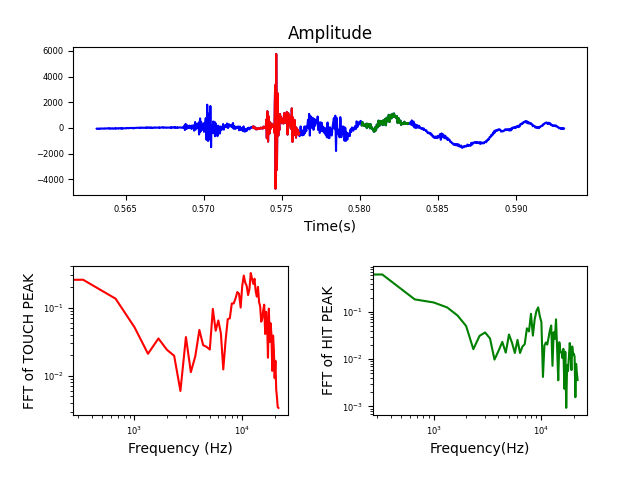
\includegraphics[width=.9\linewidth]{Images/AcCAPPCHA/feature_example}
     \caption{\footnotesize{Example of normalized FFT coefficient of the touch peak and the hit peak for an audio file of key \texttt{0}.}}\label{AcCAPPCHA:feature_example}
\end{figure}
In the third case, the touch peak and the hit peak samples, taken by the 3 ms windows, are concatenated and then the spectrogram is computed over these samples (see \myref{Figure}{AcCAPPCHA:spectrogram}). From the spectrogram, I extract a feature composed by 512 values through the use of the VGG16 convolutional neural network.
\begin{figure}[H]
     \centering
     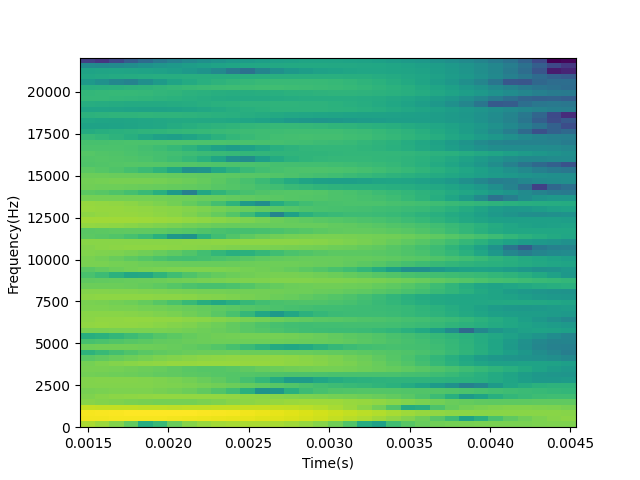
\includegraphics[width=.8\linewidth]{Images/AcCAPPCHA/spectrogram}
     \caption{\footnotesize{Example of spectrogram for an audio file of key \texttt{0}.}}\label{AcCAPPCHA:spectrogram}
\end{figure}
VG16 was pre-trained on the images of \href{http://www.image-net.org/}{ImageNet} database and I used the intermediate results from neurons, before the last fully connected layers, as feature. The reason of this approach is that a pre-trained network already extracts very well features for good classification of many labels and it can extract features better than a Convolutional Neural Network, for image classification, created from scratch.\\
The features obtained from the audio files are organized into two dataset: the training set and the test set. After the extraction of the features with one of the previous methods, I created a deep neural network from scratch.\\
Its number of input neurons is equal to the size of a feature and the number of output neurons is equal to the number of keys to be mapped. I tried to insert several hidden layers composed by different number of neurons but after changing many parameters, I decided to use only one hidden layer of 1024 neurons if the feature was obtained using the spectrograms and 100 otherwise. \\
This choice comes from the best trade-off between the accuracy (83-86\%) of the network on the test set and the correct prediction of the labels for new audio peaks obtained later during the insertion of the password. Each label associated to a key press (see \myref{Appendix}{appendix:KeyMap}), is mapped into an integer number in $[0, n-1]$ where $n$ is the number of the output neurons.\\
Each time the neural network receives a feature as input, it would return a series of floating point values (probabilities) in $[0, 1]$, one for each output neuron. The neuron, related to the highest probability, is the label predicted from the input feature. The training phase of the neural network is performed looking at the real label of each audio file and the predicted one. Thanks to the back propagation procedure, the weights of the network are modified and hence the network becomes trained. 

\subsubsection{Verification}
The verification phase is performed by AcCAPPCHA. The audio signal, recorded during the insertion of the password, is analysed and then the verification can be based on:
\begin{itemize}
\item{every audio peaks obtained using the threshold from the noise evaluation}
\item{audio peaks related to the time instants of the time correspondence}
\end{itemize}
After the selection of the previous peaks, AcCAPPCHA analyses the touch and the hit peaks and it computes the features using the approach chosen by the user at the start-up of the program, from the ones described in \myref{Section}{AcCAPPCHA:classification}. The selection of the features type is only for testing purpose and, if the CAPTCHA is released, it will be removed by using only the feature with the best results. I perform the prediction using the Neural Network trained during the classification phase. For the feature of each audio peak $f_i$, I collect the 10 most probable predicted labels in the set $Y_i=\{ {y_i}^{0}, {y_i}^{1}, ..., {y_i}^{9}\}$.\\
Then AcCAPPCHA evaluates if there exists a character correspondence by using \myref{Algorithm}{AcCAPPCHA:char_algorithm}.
If there exists a sequence of sets that "overlaps" with the characters of the password, inserted by the user, the algorithm decrees that a human performed the action. Otherwise, the user was a bot. If the verification is performed using every audio peaks, the results are very weak because it could introduce also false positives.\\
This could happens when the audio, recorded during the noise evaluation, is very flat and the audio, related to the insertion of the password, is very noisy. In this case the sequence of audio peaks, found by the character correspondence, could be composed by peaks that aren't related to all the real key presses. The main problem of this approach is caused by the missing time correspondence between a character, belonging to the final sequence, and the instant in which the same character was physically inserted by the user.\\
However, as previously mentioned, the character correspondence could also be applied after the time correspondence. In this way, \myref{Algorithm}{AcCAPPCHA:char_algorithm} would be applied on the sets of labels predicted for the audio peaks, obtained by the time correspondence. In this case, AcCAPPCHA verification becomes more accurate even if in practice character correspondence isn't very efficient because the neural network often fails in single key prediction, causing some false negatives (a human is classified as a bot).
\begin{algorithm}[h]
\DontPrintSemicolon\footnotesize
\KwIn {$\mathtt{password=(x_0, x_1, ..., x_{|password|-1})=}$ sequence related to the password, where $x_i$ is the label related to i-th character of the password typed by the user\newline
$\mathtt{Y =(Y_0,Y_1,...,Y_{n-1})=}$ sets of labels related to all the audio peaks\newline}
\KwOut {$\mathtt{true}$ if human, $\mathtt{false}$ otherwise\newline}
\BlankLine
\If{$n<|password|$}{
\textcolor{commentAlg}{//Number of found peaks lower than number of characters of the password}\;
    \BlankLine
    \Return $false$\;
    \BlankLine
}
\BlankLine
\textcolor{commentAlg}{//Search of sequence}\;
$\mathtt{i\gets} 0$\;
\For{$j\leftarrow 0$ \KwTo $n-1$}{
\BlankLine
 \If{$x_i\;\in\; Y_j$}{
 \textcolor{commentAlg}{//Character $x_i$ found in the set of labels $Y_j$}\;
    \BlankLine
    $\mathtt{i\gets} i+1$\;
    $\mathtt{j\gets} j+1$\;
    \BlankLine
 }
 \If{$i==n$}{
 \textcolor{commentAlg}{//Character correspondence found (all the characters of the password were found in $Y$)}\;
    \BlankLine
    $\mathtt{break}$\;
    \BlankLine
 }
\BlankLine
}
\BlankLine
\Return i==n
\BlankLine
 \caption{Character correspondence}\label{AcCAPPCHA:char_algorithm}
\end{algorithm}


\section{Communication between client and server}\label{AcCAPPCHA:communication_CS}
After the evaluation of the user activity, the response will be signed through ECDSA and the credentials of the client will be sent to the server if and only if the insertion of the password was performed by a human. The evaluation of the user's activity (see \myref{Section}{AcCAPPCHA:user_activity}) is performed at the client side but the server is the one that establishes if the user was a human.\\
The response of the evaluation of the user's activity, concatenated with a nonce and signed through ECDSA, is sent to the server (see \myref{Section}{inv:communication}). The use of the nonce, a unique and random generated sequence, is very important to guarantee that no replay attacks would be performed. In fact after the reception of a message from the client, the server checks if the same client has sent the same nonce before and in this case it declines the message of the client. In this way, any attacker can't reuse a message sent by a human client before.\\
The ECDSA signature can be also useful to sign HTTP data, for example a POST request, to increase the integrity of the messages and the security of the communication between the client and the server. In the testing phase I performed, I designed and implemented also a simplified version of the communication between the client and the server during the authentication service. The application was tested on the local network and the actions performed by the involved parties are described in details in the following sections (see \myref{Figure}{AcCAPPCHA:ClientServer}).
\begin{figure}[h]
\centering
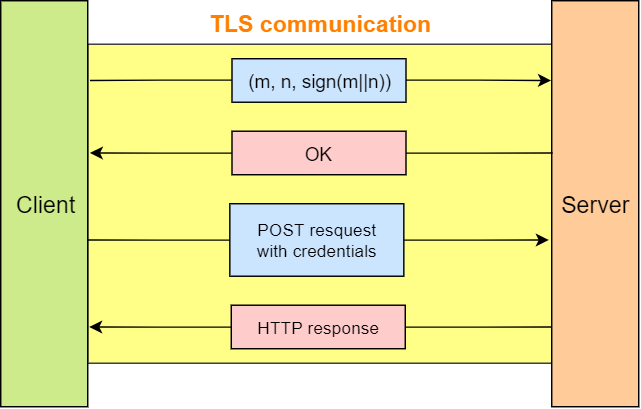
\includegraphics[width=.8\textwidth]{Images/AcCAPPCHA/client-server}
\caption{\footnotesize{Authentication between client and server using AcCAPPCHA.}}\label{AcCAPPCHA:ClientServer}
\end{figure}
\subsection{Client}\label{AcCAPPCHA:client}
The client performs the authentication following these steps:
\begin{enumerate}
\item{The client establishes the connection with the server using the Transport Layer Secure (TLS) protocol to increase the security strength of the communication between the parties;}
\item{The client sends the message $(m, n, sign(m||n))$ to the server where:
\begin{itemize}
\item{$m$ is the string with the response of the evaluation of the user's activity on the client side (\texttt{True} if Human, \texttt{False} if bot)}
\item{$n$ is the client nonce}
\item{$sign(m||n)$ is the ECDSA signature of the concatenation $m||n$ of the response and the nonce. I decided to use SHA256 as hashing function exploited by ECDSA.}
\end{itemize}
In practice, I format the message $(m, n, sign(m||n))$ in the following way to easily distinguish the portions of the message:
\begin{table}[H]
\centering\footnotesize
\begin{tabular}{|c|}
\hline
\texttt{m CRLF n sign(m||n)}\\
\hline
\end{tabular}
\end{table}
According to the basic rules in the grammar of \textbf{HTTP/1.1} (see Section 2.2 of \href{https://tools.ietf.org/html/rfc2616}{RFC 2616}), \textit{CR} is the carriage return ($\mathtt{\setminus r}$) and LF is the line feed ($\mathtt{\setminus n}$). The spaces in the format string aren't inserted in the message, if not explicitly specified with format string \textbf{SP}. The introduction of $\mathtt{\setminus r\setminus n}$ is intended to easily identify $m$ because it can be a message composed by 4 or 5 characters. However the nonce is a Universally Unique Identifier (UUID) and it has a fixed length of 16 bytes. In this way, I emulated the uniqueness of the nonce.}
\item{The client waits for the response of the server, that has the following format:
\begin{table}[H]
\centering\footnotesize
\begin{tabular}{|c|}
\hline
\texttt{response CRLF}\\
\hline
\end{tabular}
\end{table}
If the answer is equal to $\mathtt{OK\setminus r\setminus n}$, the user was a human and AcCAPPCHA will go on with the authentication step. Otherwise the user is classified as a bot and the client-side application performs again the verification, asking the user to insert the password. The maximum number of trials for a specific user is 3 and if the client reaches it, the client-side will block the next accesses to AcCAPPCHA for a fixed amount of time. In this case AcCAPPCHA can't run and it terminates immediately the execution by writing on the standard output that the user can't access to the application.}
\item{If the user was classified as a human, the client sends the credentials (username, password) to the resource \texttt{/cgi-bin/auth} of the server, using an HTTP POST request, and performs the next phases. The name of the folder \texttt{/cgi-bin} is the name of the standard path that identifies function calls. In fact \textit{auth} is the name of the function that server will call during the authentication phase. This naming approach was used very much in the past to separate functions code from pure HTML code. The password is not sent directly but it's hashed using SHA512. The POST request sent by the client has the following format:\\
\begin{table}[H]
\hspace{2cm}\centering\footnotesize
\begin{tabular}{|l|}
\hline
\texttt{POST /cgi-bin/auth HTTP/1.1} $\mathtt{\setminus r\setminus n}$\\
\texttt{Host: SP foo.example CRLF}\\
\texttt{Content-Type: SP application/x-www-form-urlencoded CRLF}\\
\texttt{Content-Length: SP SIZE CRLF CRLF}\\
\texttt{user = USERNAME $\mathtt{\&}$ pwd = HASHEDPWD}\\
\hline
\end{tabular}
\end{table}
where \textbf{SIZE}, \textbf{USERNAME} and \textbf{HASHEDPWD} are replaced respectively with the size of the HTTP body, the username of the client and its password hashed with SHA512. The format of the POST request follows again the grammar of HTTP/1.1, specified in \href{https://tools.ietf.org/html/rfc2616}{RFC 2616}).
}
\item{The client waits for the HTTP response of the server, containing HTML code as body. Then the client saves the code on the file system and opens the default web browser to show the HTML page received. The HTML code is intended to show 3 possible scenarios: the user was correctly logged in, the user inserted wrong password, the username wasn't already stored on the server database. In the last two scenarios, AcCAPPCHA will ask again the credentials to the user, waiting for the password or both the username and the password. The client can insert wrong credentials for at most 3 times. If the limit is reached, the access of the user to AcCAPPCHA is blocked.}
\end{enumerate}
When the user is blocked because the client inserted wrong credentials or a bot was detected, the client-side of AcCAPPCHA stores the datetime in a file called \texttt{block.txt}. At every start-up of AcCAPPCHA on the client side, the program checks if a fixed amount of time was passed from the stored datetime. If the block period is already elapsed, the file \texttt{block.txt} is removed by the client, otherwise it isn't touched and it will be used for future checks. During the testing phase, I used a block period of 100 seconds but in practice it should be bigger.

\subsection{Server}
The server performs the authentication of the client following these steps:
\begin{enumerate}
\item{The server establishes the connection with the client, after his request, using the TLS protocol to increase the security strength of the communication between the parties;}
\item{The server receives the message $(m, n, sign(m||n))$ and it checks the integrity of the message. To do it, the server decrypts the ECDSA signature using the client's ECDSA public key and it compares the result with \textit{m||n}. If the comparison fails, the server replies $\mathtt{No\;integrity\setminus r\setminus n}$ to the client.}
\item{If the previous comparison has a positive response, the server checks if the nonce was already used by the same client. If this happens, the server thinks that an attacker is performing a replay attack and the server replies $\mathtt{NO\setminus r\setminus n}$ to the client. If the nonce wasn't already used by the client, it will be stored in a dictionary to monitor clients activity. Each entry of the dictionary is composed by:
\begin{itemize}
\descItem{Key: IP address}{It is the IP address of the client and it is a simplification of the information that could identify a client. For example the client could be associated also to port number used to make the request, the Operating System on which the AcCAPPCHA was running on the client-side or other useful parameters.}
\descItem{Value: list of nonces}{Every time a client performs a new verification request on the server, the nonce used is added to the list related to its key in the dictionary.}
\end{itemize}
}
\item{If the nonce was used for the first time by the client, the server checks the value of the response received by the client. If the response is \texttt{True}, the server replies $\mathtt{OK\setminus r\setminus n}$ otherwise $\mathtt{NO\setminus r\setminus n}$. If some error occurs it sends $\mathtt{ERROR\setminus r\setminus n}$ to the client. In the last two cases, the server doesn't perform the following steps.}
\item{If the server doesn't terminate, it waits for the POST request from the client and analyses it to perform the authentication service. The server replies to the client with an HTTP 1.1 response with several possible status codes:
\begin{itemize}
\item{\textbf{501 (}Not implemented\textbf{)}\\
If the request is not a POST (e.g. GET)}
\item{\textbf{400 (}Bad Request\textbf{)}\\
If the number of the parameters in the POST body is different from 2 (username and password).}
\item{\textbf{200 (}OK\textbf{)}\\
If the number of the parameters in the POST body is equal to 2, the server will reply with an HTTP response with a body content depending on several cases:
\begin{itemize}
\descItem{The user isn't in the database}{the server sends the following HTML code if the specified username isn't already stored in the database.
\begin{table}[H]
\hspace{2cm}\centering\footnotesize
\begin{tabular}{|p{6cm}|p{0.5cm}c}
\cline{1-1}
\texttt{\key{<!DOCTYPE html>}}&\multirow{7}{*}{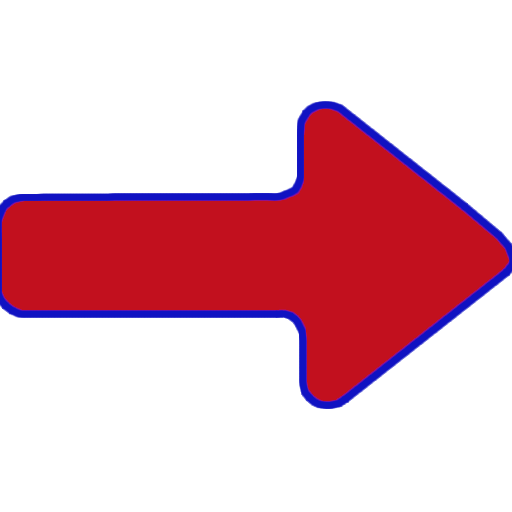
\includegraphics[width=0.5cm]{Images/arrow}}&\multirow{7}{*}{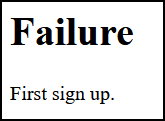
\includegraphics[scale=0.8]{Images/AcCAPPCHA/no_db_html}}\\
\texttt{\key{<html>}}&&\\
\texttt{\hspace{0.5cm}\key{<body>}}&\\
\texttt{\hspace{1.0cm}\key{<h1>}Failure\key{</h1>}}&&\\
\texttt{\hspace{1.0cm}\key{<p>}First sign up.\key{</p>}}&&\\
\texttt{\hspace{0.5cm}\key{</body>}}&&\\
\texttt{\key{</html>}}&&\\
\cline{1-1}
\end{tabular}
\end{table}
}
\descItem{The password is wrong}{the server sends the following HTML code if the hashed password, sent by the client, isn't equal to the one stored in the database for the username, specified by the client.
\begin{table}[H]
\hspace{2cm}\centering\footnotesize
\begin{tabular}{|p{6cm}|p{0.5cm}c}
\cline{1-1}
\texttt{\key{<!DOCTYPE html>}}&\multirow{7}{*}{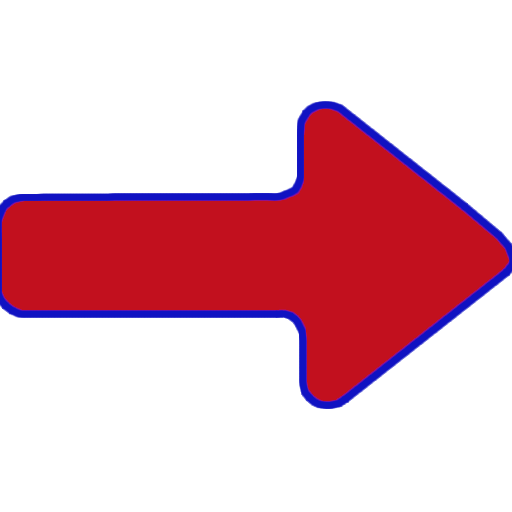
\includegraphics[width=0.5cm]{Images/arrow}}&\multirow{7}{*}{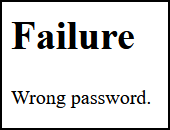
\includegraphics[scale=0.8]{Images/AcCAPPCHA/failure_html}}\\
\texttt{\key{<html>}}&&\\
\texttt{\hspace{0.5cm}\key{<body>}}&&\\
\texttt{\hspace{1.0cm}\key{<h1>}Failure\key{</h1>}}&&\\
\texttt{\hspace{1.0cm}\key{<p>}Wrong password.\key{</p>}}&&\\
\texttt{\hspace{0.5cm}\key{</body>}}&&\\
\texttt{\key{</html>}}&&\\
\cline{1-1}
\end{tabular}
\end{table}
}
\descItem{The user correctly logged in}{the server sends the following HTML code if the specified username exists in the database and the hashed password stored in the database is equal to the one received in the POST request.
\begin{table}[h]
\hspace{2.5cm}\centering\footnotesize
\begin{tabular}{|p{6cm}|p{0.5cm}c}
\cline{1-1}
\texttt{\key{<!DOCTYPE html>}}&\multirow{7}{*}{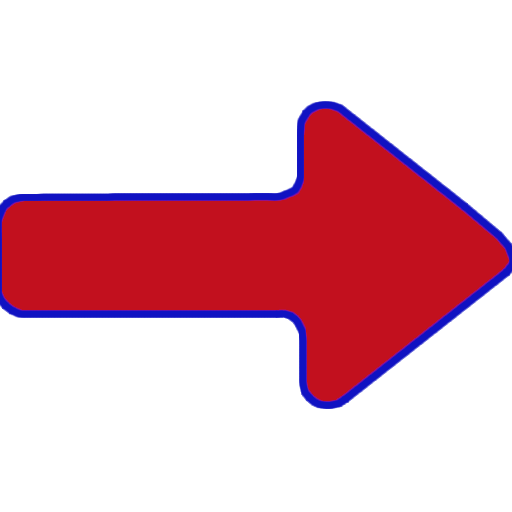
\includegraphics[width=0.5cm]{Images/arrow}}&\multirow{7}{*}{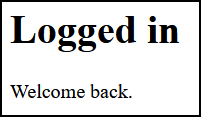
\includegraphics[scale=0.8]{Images/AcCAPPCHA/logged_html}}\\
\texttt{\key{<html>}}&&\\
\texttt{\hspace{0.5cm}\key{<body>}}&&\\
\texttt{\hspace{1.0cm}\key{<h1>}Logged in\key{</h1>}}&&\\
\texttt{\hspace{1.0cm}\key{<p>}Welcome back.\key{</p>}}&&\\
\texttt{\hspace{0.5cm}\key{</body>}}&&\\
\texttt{\key{</html>}}&&\\
\cline{1-1}
\end{tabular}
\end{table}
}
\end{itemize}
}
\end{itemize}
}
\end{enumerate}
\subsection{Database}
The database, created to simulate the search of a username by the server, was made using PostgreSQL. I could store all the information in a simple text file or a csv file but I decided to use this approach to be more flexible and to emulate the integration of AcCAPPCHA in more complex web applications.\\
The database is composed by a single table \texttt{CloudUser} that stores information about the users identities, that are usually asked to the clients during the sign up phase. The creation of the database table was performed using the following instructions:
\lstset{basicstyle=\footnotesize,breaklines=true}
\lstinputlisting[language=SQL]{../Code/PC/dat/db/db_creation.sql}
I created several domains to manage the format of some information of the user. For example the password is a string of 128 characters because each password is hashed using SHA512 and then stored as a string of hexadecimal digits.
Then I populated the dataset with some entries, related to fake users, only for testing purpose. An example of the query that I use to insert information about a user is reported next:
\vspace{0.5cm}
\begin{lstlisting}[language=SQL, showstringspaces=false]
INSERT INTO CloudUser (Name,
                       Surname,
                       Username,
                       Email,
                       Sex,
                       Password)
                       
VALUES ('Raffaele', 
        'Di Nardo Di Maio', 
        'RaffaDNDM', 
        'example1@gmail.com', 
        'Male',
        HASHPASSWORD);
\end{lstlisting}
During the insertion, \texttt{HASHPASSWORD} was replaced by the string of 128 characters corresponding to the hashed password in hexadecimal format.

\subsection{Encryption Keys}
The creation of the TLS socket for the communication between the client and the server is done by using keys and certificates created thanks to the following bash instructions:
\vspace{0.3cm}
\begin{lstlisting}[language=bash, showstringspaces=false, tabsize=4]
openssl req -new -x509 -days 365 -nodes -out client.pem
		-keyout client.key
\end{lstlisting}
\begin{lstlisting}[language=bash, showstringspaces=false, tabsize=4]
openssl req -new -x509 -days 365 -nodes -out server.pem 
		-keyout server.key
\end{lstlisting}
OpenSSL is a open-source implementation of TLS/SSL protocols and, thanks to the option \texttt{-x509}, you can display certificates and also access to many signing protocols.
In particular, in the previous bash instructions, a X.509 Certificate Signing Request (CSR) is generated and signed for both the parties.\\
Thanks to \texttt{-nodes} the private key is created and not encrypted. The certificates are stored respectively in \textit{server.pem} for the server side and \textit{client.pem} for the client and they are valid for 365 days. The private keys are stored, using the \texttt{-keyout} option, in the files \textit{client.key} and \textit{server.key}.\\\\
The keys, used in ECDSA signing and verification, were created as follow from the Python language instead of using a bash tool:
\vspace{0.3cm}
\begin{lstlisting}[language=python, showstringspaces=false, tabsize=4]
from ecdsa import *
from hashlib import sha256

PRIVATE_KEY = SigningKey.generate(curve=SECP256k1,
                                  hashfunc=sha256)

with open('ecdsa.key', 'w') as private_pem:
	private_pem.write(PRIVATE_KEY.to_pem().decode())

PUBLIC_KEY = PRIVATE_KEY.get_verifying_key()

with open('ecdsa.pem', 'w') as public_pem:
	public_pem.write(PUBLIC_KEY.to_pem().decode())
\end{lstlisting}
In this case the private key, used to sign a message from the client, was computed on the curve \texttt{SECP256k1} usually used in Bitcoin applications.